
\documentclass[natbib,referee]{svjour3}

\smartqed  % flush right qed marks, e.g. at end of proof


% PACKAGES
% ------------------------------------------------------------------------------

\usepackage{simplemargins}
\usepackage{textcomp}
\usepackage{amsbsy}
\usepackage[dvipsnames]{xcolor}

\usepackage{graphicx}
\usepackage[pdftex,bookmarks=false]{hyperref}
\usepackage{float}


% LINKS
% ------------------------------------------------------------------------------

\hypersetup{
    pdfpagelayout=OneColumn,
    colorlinks = true,
    urlcolor   = blue,
    citecolor  = blue,
    linkcolor  = blue
}
\urlstyle{same}


% ADDITIONAL COMMANDS
% ------------------------------------------------------------------------------

\newcommand{\myrevision}[1]{\textcolor{Black}{#1}}
\settopmargin{1.2in}
\setleftmargin{.9in}
\setrightmargin{1in}
\setbottommargin{.2in}


% JOURNAL NAME
% ------------------------------------------------------------------------------

\journalname{Note Decided}


% MAIN DOCUMENT STARTS
% ==============================================================================

\begin{document}


% TITLE
% ------------------------------------------------------------------------------

\title{An investigation on the applicability of equivalent linear-method ideas in three-dimensional models for earthquake ground motion simulation}
\titlerunning{Equivalent linear method in 3D}


% AUTHORS
% ------------------------------------------------------------------------------

\author{%
    Naeem Khoshnevis \and 
    Ricardo Taborda \and
    Doriam Restrepo 
}

% \authorrunning{N.~Khosh} % if too long for running head

\institute{
    N. Khoshnevis
       \at
        Center for Earthquake Research and Information\\
        The University of Memphis, Memphis, TN 38152, U.S.A.\\
        \email{nkhshnvs@memphis.edu}\\
    R. Taborda 
        \at
        Center for Earthquake Research and Information\\
        and Department of Civil Engineering
        The University of Memphis, Memphis, TN 38152, U.S.A.
    \and
    D. Restrepo
        \at
    Department of Civil Engineering, University of EAFIT, Colombia
}

\date{Received: date / Accepted: date}

\maketitle

\begin{abstract}
    %
There is ample evidence about the effects and importance of the nonlinear response of sediments during strong earthquake ground motion. Depending on the modeling scales and the level of knowledge about material properties, these effects can be estimated by means of nonlinear or equivalent linear methods. While the former is well-founded in theoretical grounds and the known (experimental) behavior of geomaterials, the latter is based on simplified assumptions. The equivalent linear method is, nonetheless, more broadly used in engineering practice due to its simplicity and effectiveness. In principle, this method is limited to problems under shear-deformation and the one-dimensional (1D), vertical propagation of seismic waves through horizontal layers. Realistic, nonlinear soil-modeling approaches, on the other hand, while more appropriate for general applications, are restricted to highly specialized studies. This is mostly due to the required level of knowledge about material properties and the entailed computational overhead. As a result, three-dimensional (3D) nonlinear earthquake ground motion simulations at regional scales are seldom done. In this study we explore the applicability of equivalent linear-method ideas in 3D earthquake ground motion simulations at a regional scale. We implement a version of the linear equivalent method in 3D using a finite element software for wave propagation simulations, and start by testing our implementation under 1D (shear) wave propagation conditions. We then follow a careful, progressive approach to study the applicability of well-known shear modulus degradation and damping ratio curves to update material properties during the iterative simulation process, as we increase the geometrical complexity of the models from 1D to 3D conditions. We compare the results obtained with nonlinear solutions, analyze the qualitative effectiveness of the approach to approximate the known effects and characteristics of nonlinear behavior in 3D basins during earthquake ground shaking, and draw conclusions from these comparisons to inform possible paths forward.
    \keywords{Equivalent Linear Method \and 
3D ground motion simulation 
}
\end{abstract}



\section{Introduction}

Near surface low velocity layer has a significant effect on seismic waves frequency content and amplitude. Amplification, deamplificaiton and shift in resonant frequency are important factors in designing structures and buildings. Devastating damage after Micheocan, Mexico (1985), Kalmat, Greece (1989), Loma Perieta, California, USA (1989), Roodbar-Manjil, Iran (1990) and other earthquakes highlighted the importance of comprehensive site response analysis in engineering practices. Fully nonlinear and equivalent linear analyses are used to consider the nonlinear behavior of soil during earthquake. Among those the latter lend itself in engineering practices. Fully nonlinear site response analysis is important to estimate soil behavior during earthquake and are necessary to capture phenomena such as irreversible deformations and pore pressure coupling, however, its usage in standard engineering practice is relatively limited \citep{Assimaki2008quantifying}. The main reason is lack of soil data.  Nonlinear soil analysis needs parameter which is not available for all site even for well stablished KiK-net sites \citep{Kaklamanos2013critical}. Elaborate constitutive laws require numerous parameters that need to be determined through laboratory and  field techniques and are therefore associated with considerable cost and effort in design practice because they require both detailed site characterization and significant engineering time for analysis \citep{Assimaki2008quantifying}.

The equivalent linear method is perhaps the most widely employed approach for strong motion site response predictions in engineering practice\citep{Assimaki2008quantifying}. The idea of replacing a nonlinear system by an "equivalent" linear system whose behavior will be an approximation to that of the nonlinear system was first introduced by \citet{jacobsen1930steady}. He compared the various criteria of equivalence with exact solutions for specific problems,  and with experimental results, He concluded that the most useful criterion is that of the equivalence of energy dissipated per cycle. In other study, \citet{Kryloff1943} replaced the general nonlinear equations' damping and spring constant with modified values so that the solution of the linear equation is an approximate solution of the nonlinear equation. \citet{Hudson1965}  defined an equivalent viscous damping coefficient by equating the energy loss per cycle in a hysteretic system to energy loss per cycle in the corresponding small amplitude linear system. The new damping coefficient resulted in accurate calculations of the maximum amplitude of resonant vibrations in hysterestic systems that are strongly nonlinear.  Based on these successful applications of equivalent linear analyses, \citet{Idriss1968} proposed the implementation of the equivalent linear method in site response analysis. The procedure involves the determination of an equivalent linear modulus, $G_{eq}$, and an equivalent damping ratio $\lambda_{eq}$ for use in a linear elastic solution. They proposed to use other numerical methods (e.g., Finite-Element method) in case of  non-horizontal boundaries, and non horizontal excitations. \citet{Idriss1970} summarized the available data of shear modulus and damping for different soil and site and also different tests  and  developed  shear moduli and damping ratios for soils with different parameters. Integrating all these theory and laboratory results,  \citet{Schnabel1972a} developed a software known as SHAKE to conduct a 1D site response analysis for horizontal layers. Equivalent linear methods because of simplicity, need for less input parameters, and computationally efficiency have been used in many different engineering practice and site response analysis. Two decades later, \citet{Idriss1992}, developed the modified version of SHAKE and called it SHAKE91. The modified version of SHAKE was suitable for personal computers. The program computes the response of  semi-infinite horizontally layered soils deposit overlying a uniform half-space subjected to vertically propagating shear waves. The analysis is done in the frequency domain, and, therefore, for any set of properties it is linear analysis. SHAKE91 still is in use in engineering practice and research. Since then, equivalent linear method, specifically shake is used in numerous site response analysis. SHAKE is the most widely used analysis package for 1D site-specific response calculations \citet{Assimaki2008quantifying}. \\
Many other packages were developed to conduct site response analysis using equivalent linear method, however, the general idea is the same. (give some references).


Equivalent linear method are mostly used through 1D site response analysis. However, the idea is used in 2D and 3D simulation to approximate the nonlinear soil behavior. \citet{Lysmer1974} and \citet{Lysmer1975} were among the initial attempts to include the equivalent linear method in 3D simulation. They developed a computer program (LUSH and FLUSH) to approximate 3D analysis of soil-structure interaction problems mostly for nuclear power plant structures. A control motion,  specified at some point in the free-field surface profile, can be deconvolved to determine the corresponding motions at some depth, such as a soil-rock interface. The motion computed at this depth is used as input to a finite element model of the soil structure system. In each iteration the analysis is linear but the soil properties are adjusted from iteration to iteration until the computed strains are compatible with the soil properties used in the analysis. It mostly needs 3 to 5 iterations to converge. They proposed a method to define the effective strain based on current strain level and input acceleration level. In another study, \citet{Lysmer1981} developed a system for 3D soil-structure interaction to analyze the horizontal viscoelastic layers on horizontal viscoelastic half space through accepting a combination of incoming body wave and horizontal surface wave for standard 3D finite element structures. They approximated the nonlinear effects by an equivalent linear method.  

Full 3D nonlinear soil simulation with addressing the 3D aspects present in a region where soil nonlinearities are combined with source path and basin effects is studied from different perspective. \citet{Xu2003} reported the development and application of a parallel numerical methodology for simulating large-scale earthquake-induced ground motion in highly heterogeneous basin whose soil constituents can deform nonlinearly . They used an idealized basin with an arbitrary seismic excitation. The basin material is modeled as Drucker-Prager elastoplastic materials. Their simulations show that elastoplastic soil behavior results in overall reduction of the ground acceleration through the basin. The significant reduction in peak resonance was reported, however, there was small changes in dominant frequency. \cite{Dupros2010} presented finite-element numerical simulation of seismic wave propagation in nonlinear inelastic geological media. They used Mohr-Coulomb model for simulating the nonlinear behavior of soil. They conducted the simulation within French Riviera up to 0.5 Hz. They observed increment in peak ground displacement and reduction in peak ground velocity and acceleration due to nonlinear soil behavior. \citet{Taborda2010} implemented vonMises and Drucker-Prager models in 3D ground motion simulation FEM code called Hercules.  two cases for the elastoplastic ground response of the valley for moderate and severe nonlinearities.  (Also include Taborda Bielak Restrepo 2012).

As mentioned earlier nonlinear site response analysis needs elaborate set of soil parameters which is not available for all places. The analyses become more computationally challenging in 3D simulation. In this paper we propose using equivalent linear method in 3D ground motion simulation from source to site without further pre- or post-processing. We compare the fully nonlinear and equivalent linear simulation results and discuss the appropriate range of parameters that needs to be consider. In the following section we discuss the equivalent linear solution steps and implementation in 3D ground motion simulation. Later on we discuss the fully nonlinear solutions. We test the idea on different site, source, and magnitudes. We also use the simulation for realistic simulation. Our results show that the equivalent linear method have good agreement with fully nonlinear solution in terms of PGV, PGA, and their frequency contents. It has also a good agreement with response spectra. Regarding the significantly low computational cost, and lower number of input values, equivalent linear method in 3D simulation can be a good alternative for fully nonlinear methods in large scale ground motion simulation for considering nonlinear soil behavior. 






%The most common manifestations of inelastic soil behavior involve the reduction in shear wave velocity and the increase in soil damping with increasing load (Hardin and Drnevich, 1972). Simulations of nonlinear earthquake response be-gan in the late 1960s. These early studies were con- ducted for horizontally layered soils and vertically incident waves, by either an equivalent linear or a direct nonlinear method. These are the main meth- ods that are still used today in engineering practice. In the equivalent linear method, the soil response is evaluated in an iterative manner. First, trial values for average strain are chosen, then soil properties are de- termined in accordance with the trial values of strain, and finally the response of the model is calculated. If the calculated strains differ significantly from the trial values, the cycle is repeated (Idriss and Seed, 1968; Schnabel et al., 1972).While one-dimensional (1D) simulations can yield reasonable estimates of nonlinear effects under ver- tically incident seismic excitation, they cannot rep- resent the effects of surface waves and basin effects. However, observations from many recent strong motion events have demonstrated that nonlinear soil behavior strongly affects the seismic motion of near-surface deposits, resulting in shear wave velocity reduction, irreversible settlements, and in some cases pore-pres- sure build-up leading to liquefaction.The effect of the nonlinear constitutive law on acceleration is much more difficult to interpret; the global trend is to add an important high frequency content (in agreement with [43]) and to increase peak ground acceleration after the shear wave portion: see I. Beresnev, K. Wen, Nonlinear soil response ? a reality?, Bull Seism. Soc. Am. 86 (6) (1996) 1964?1978.




\section{Nonlinear Soil Behavior and Strain Level}

Nonlinear soil behavior is in direct relationship with the strain level that is imposed during the loading process. \citet{Ishihara_1996} classified the shear strain level into four categories, which can be represented through 3 different models. Fig.~\ref{fig:ishihara_fig_3p1} represents different strain level and appropriate models to present them.


\begin{figure}[H]
    \centering
    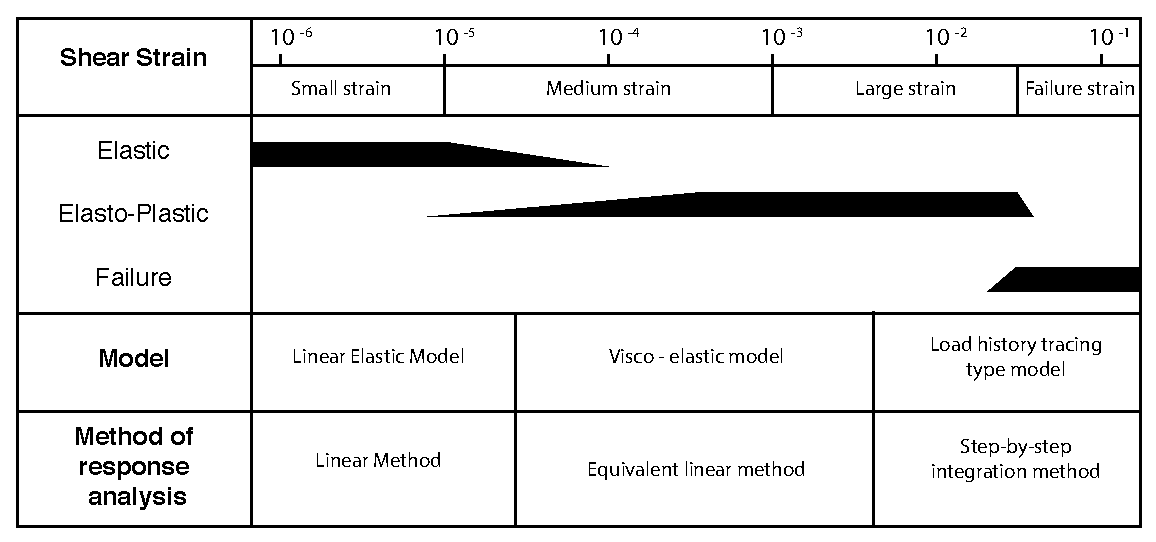
\includegraphics[width=300px]{figures/pdf/ishihara_fig_3p1.pdf}
    \caption{Modeling soil behavior based on strain level. The original figure is provided in  \citet{Ishihara_1996}}
    \label{fig:ishihara_fig_3p1}
\end{figure}



When soil behavior is expected to stay within the range of the small strain, the use of an elastic model is justified and the shear modulus is a key parameter to properly model the soil behavior. In this situation the intrinsic attenuation due to internal friction of the soil materials is considered through anelastic simulation. \citet{Assimaki2000} found the linear threshold of strain about $10^{-5}$. In cases of medium range of strains (below the level of $10^{-3}$) the soil behavior becomes elasto-plastic and the shear modulus tends to decrease with increasing shear strain, and during the cycles of load application the energy dissipation occurs. In this case the energy dissipation is mostly rate-independent and of hysteric nature, and the damping ratio can be used to represent the energy absorbing properties of soil. Due to low strain level (below the level of $10^{-3}$) the soil properties and damping level do not change with progression of load application. This kind is called non-degraded hystersis type. Linear viscoelastic models can be used to represent the soil characteristics in this strain level. For the strain level larger than about $10^{-2}$, soil properties tend to change appreciably not only with shear strain by also with the progression of cycles. This behavior is called degraded-hysteresis type. Representing the characteristics of soil behavior in this strain level needs establishing a constitutive law in which stress-strain relations can be specified at each step of loading, unloading, and reloading phases. 

Also in many other studies for 1D programs equivalent linear method and nonlinear method are used to compare the results and give an estimation about the strain boundaries that equivalent linear method remains accurate.

 \citet{Kaklamanos2015} performed a comprehensive linear, equivalent linear, and nonlinear site response analyses on 191 ground motions record at six validation site in the Kiban-Kyoshin network (KiK-net) of vertical seismometers arrays in Japan. They used linear, Equivalent linear and, fully nonlinear methods. They find that at peak shear strains from 0.01\% to 0.1\% linear site response models fail to accurately predict short-period ground motion; equivalent linear and nonlinear models offer a significant improvement at strains beyond this level, with nonlinear models exhibiting a slight improvement over equivalent-linear models at strains greater than approximately 0.05 \%. They also realized that the performance of the equivalent linear model is heavily dependent on the assumed modulus-reduction and damping relationships. 

\citet{Kim2013site} analyzed nine stations record during the 11 March 2011, Mw = 9.0 Tohoku-Oki earthquake to study the effect of long duration earthquake on site response analysis. They used 16 earthquakes and the one dimensional analysis code, DEEPSOIL. The response spectra captured by equivalent linear (ELA) and nonlinear (NL) approaches are similar for smaller earthquakes because of smaller maximum strain. For stations with maximum strain larger than 0.3\% the difference between ELA and nonlinear site response analysis is significant. 

\citet{Kaklamanos2013critical} used Kiban-Kyoshin network (Kik-net) downhole array data in Japan to analyze the accuracy (bias) and variability (precision) resulting from common site response modeling assumptions. They preformed linear and equivalent linear site response analysis at 100 KiK-net site using 3720 ground motion ranging from weak to strong. They found that the max shear strain in the soil profile, the observed peak ground acceleration at the ground surface, and the predominant spectral period of the surface ground motion are the best predictions of where evaluated models become inaccurate and/or imprecise. Linear analysis become inaccurate in predicting spectral acceleration between 0.01\% and 0.1\% shear strain for periods less than 0.5s ($f  > 2 Hz$). At spectral periods of $(T > 0.5 s)$ there is no noticeable nonlinear soil behavior. They concluded that when $\gamma_{max} > 4 \%$ the equivalent linear formulation generally under predicts ground motions for $T < 0.5 s$. For large ground motions (particularly for shear strain > 0.4 \%) SHAKE over predicts the amount of nonlinearity that actually occurs particularly at high-frequencies. 

\citet{Carlton2016comparison} compared the results of ELA and NLA. They found that in $\gamma_{max}$ greater than 0.04\% to 1.0\% there are non-negligible differences between ELA and NLA. They developed some criteria to estimate the $\gamma_{max}$ ELA before conducting the site response analysis. To do that they used 189 ground motions, nine hypothetical sites and seven actual sites. They found that for $\gamma_{max}$ ELA <0.003\% the soil behaves linearly so the difference between ELA and NLA is negligible. They found that the trend for  $\gamma_{max}ELA > 0.003\%$ is due to two opposite effects. ELA over damp ground motions for shear strain less than the effective shear strain, which reduces the total energy in the ground motion. However, for shear strains larger than the effective shear strain, ELA use smaller damping than NLA, which allows more energy to propagate to the ground surface. They found that ELA tend to predict more peaked response spectra than NLA, with longer amplification near the natural site period. They found the for period longer than 2 sec there is little difference at long periods because long period seismic waves are not as affected as short period seismic waves by shallow soft soil layers that usually experience the greatest nonlinear effects. These results are similar to \citet{Kaklamanos2013,Kim2013site} who found negligible nonlinear effects for period longer than 0.5s and 1s, respectively. They found that the best predictor of difference of ELA and NLA is the maximum shear strain induced in the soil column in ELA.

\citet{Yee2013elastic} presented a procedure to more realistically represent the large strain portion of backbone curves by asymptotically approaching the shear strength at large strains, which removes strain localization for this application and provides reasonable matches of observed and computed ground motions. They used main shock and after shock surface to rock transfer function to study the resonant frequency shift. They used ground response analyses to predict one-dimensional shear wave propagation through the soil column. They used EQL and Nonlinear method. They performed both methods in DEEPSOIL. For NL they used hyperbolic backbone curve. They proposed to adjust the soil backbone curve to transition toward a specific shear strength at large strains while preserving the small strain behavior from modulus reduction curves. They increased the small-strain material damping from laboratory-based values (near $D_{min}=1\%$) to higher level of $D_{min}=2\% and 5\%$ largely solve the problem of over prediction of high frequency ground response. They adjusted the shear strength degradation. Adjusted back bone curve could capture the shear strength at larger strains and improve the results.\\




\section{Draw backs of equivalent linear method}

All site response analyses are burdened with significant uncertainties in the parameters, models, and methodologies. 
Although equivalent linear method in practice is the most used method, however, like many other methods it has advantages and disadvantages. In this section we will discuss these factors. Equivalent linear method, in nature, is a linear process. Therefore, it does not have nonlinear displacement. Consequently the method is not good for studying permanent displacement due to nonlinear soil behavior. Also as mentioned before, for large strain levels that can affect the damping ratio and shear modulus with progression of cycles in load application, the equivalent linear method is not a good approach. Equivalent linear method is good for estimating long-period (low frequency) motions, however, it is not good for high frequency motions. The reason for this could be using the maximum strain or a factor of maximum strain to adjust the values. Maximum strains are results of long period motions so the results are accurate for them \citep{Kaklamanos2013critical}. 
As I mentioned above, the equivalent linear method has an overdamping issue for high frequency motions. \citep{Sugito1994frequency,Joyner1998equivalent,Assimaki2002equivalent,Park2008rate} worked on the high frequency over damping issue. However, the recommended details are to much complicated that is not in engineering practice yet and people prefer to do nonlinear site response analysis rather than that. \citet{Assimaki2008quantifying} suggests when the rock-outcrop (input) peak ground acceleration (PGA) exceeds 0.2g for soft (NEHRP class E) sites, fully nonlinear analysis is necessary. \citet{Kim2013site} found that the accuracies of equivalent linear model and nonlinear models were generally similar, but the prediction deviate when maximum shear strains exceed 0.3\%. \citet{Yee2013elastic} found that equivalent linear and nonlinear models offer similar predictions for maximum shear strains up to 0.2\%, but that prediction deviate at greater strains. When shear strains in the soil exceed some critical level, the equivalent linear approximation becomes inadequate, and fully nonlinear site response analysis are needed to accurately predict surface ground motion. See following references: \citep{Assimaki2008quantifying,Kwok2008,Kaklamanos2013critical,Kim2013site,Yee2013elastic,Matasovic2010,Hashash2016deepsoil}\\

While, however, nonlinear models are necessary when large strains and permanent displacements are expected, their prediction accuracy depends on the constitutive material law that governs soil behavior. Elaborate constitutive laws require numerous parameters that need to be determined through laboratory and field techniques and are therefore associated with considerable cost and effort in design practice because they require both detailed site characterization and significant engineering time for analysis \citep{Assimaki2008quantifying}.

Despite the effectiveness of the approach for the analysis of relatively stiff sites subjected to immediate levels of strain $(<10^{-3})$, however, the equivalent linear method has been shown to over estimate the peak ground acceleration for large events and artificially suppress the high frequency components when applied for the analysis of deep sites \citep{Assimaki2008quantifying}.

An alternative methodology that accounts for the frequency dependence of strain amplitudes and associated dynamic soil properties has been proposed by \citet{Assimaki2002equivalent}, and it has been shown to yield more satisfactory results for deep sedimentary deposits; the applicability of the alternative formulation, however, is still limited to the medium strain levels (See \citet{Assimaki2008quantifying}).

\citet{Cramer2004memphis} generated a suite of seismic hazard maps for Memphis, Shelby county, Tennessee that account for the site response of sediments in the Mississippi embayment (ME). They showed that SHAKE91 over damp the high frequency components of motion. Nonlinear methods are necessary to capture phenomena such as irreversible deformations and pore pressure coupling \citep{Assimaki2008quantifying}.


%Engineers often perform ELA rather that NLA because of their simplicity of use and low computational requirements \citep{Matasovic2012practices}
%\citet{Yee2013elastic,Tsai2009learning,Elgamal2001dynamic} suggested that the soil damping derived from laboratory testing may be too low to accurately reflect in situ damping behavior. The reason for these damping misfits are unknown but are likely related to modeling a three dimensional system in one dimensional, which necessarily omits complexities that may introduce additional damping to the site response.





\section{Equivalent Linear Method}

The most common manifestations of inelastic soil behavior involve the reduction in shear wave velocity and the increase in soil damping with increasing load. The technical implementation for one dimensional domain is presented in numerous sources \citep[e.g.,][]{Kramer1996geotechnical}. In three dimensional domain we consider the following steps: First we run the simulation and extract the strain level of each element. Then we compute the effective strain for each time step. The computation of effective strain will be discussed later. We keep the maximum effective strain through the simulation time. Based on effective strain we update the material damping and shear modulus. We repeat the iteration up to 10 times. For a time being we do not related the simulation to the convergence of strain level, however, our results represent a very good agreement (convergence) after 3-5 iteration. The convergence factor may vary with increasing geological complexity of the domain and source slip function and frequency. Fig.~\ref{fig:equivalent_linear_flowchart} presents the equivalent linear work flow. 

\begin{figure}[H]
    \centering
    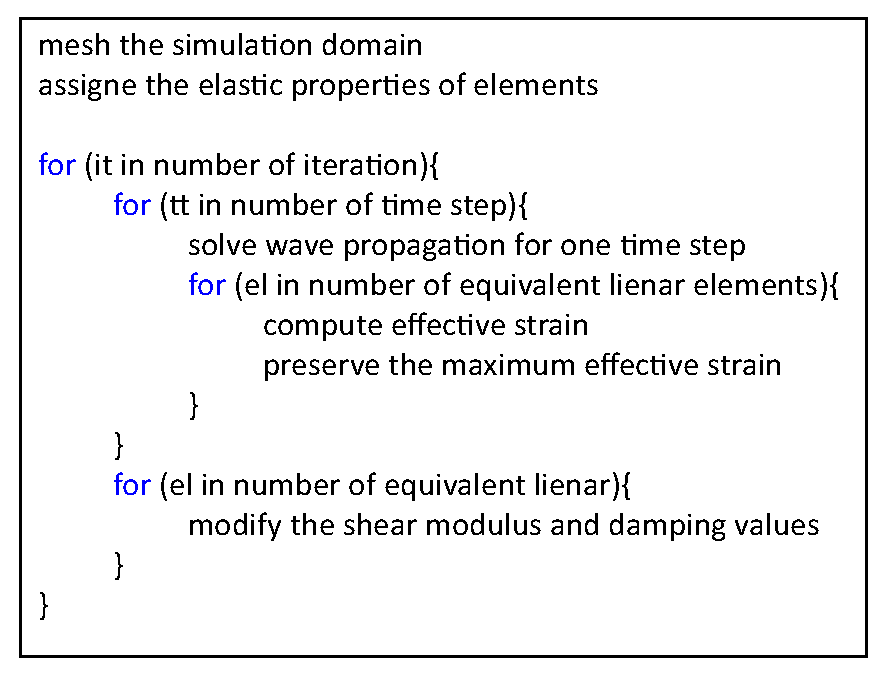
\includegraphics[width=300px]{figures/pdf/equivalent_linear_flowchart.pdf}
    \caption{Equivalent linear flowchart}
    \label{fig:equivalent_linear_flowchart}
\end{figure}


\subsection{Effective Strain}

Determination of effective strain is the most important part of equivalent linear method. In 1D simulations the effective strain is related to the shear strain of the elements (or soil layer in case of frequency domain analysis) with some modification factor. The maximum strain level of typical earthquake motion can happen at a few spikes in the record. Therefore, the maximum strain level should not be dominant value in determining the effective strain. In literature effective shear strain is defined as 50 ~ 70\% of the maximum shear strain. This value mostly is considered as 65\% \citep{Kramer1996geotechnical}.  \citet{Idriss1992} proposed to use 

\begin{equation}
R_{\gamma} = \frac{M-1}{10}
\end{equation}

 relation for determining the effective shear strain. Where M is the magnitude of earthquake. The fact that effective shear strain is related to the incoming force is also addressed in \citet{Lysmer1975}. They proposed to consider a control motion (which could be a station at rock outcrop) and define and extra value for effective strain as 
 
 \begin{equation}
c = \frac{max|\ddot{y}(t)|}{RMS(\ddot{y}(t))}
\end{equation}

where $\ddot{y}(t)$ is the control motion and RMS is root mean square function. $c$ is the additional scaling factor for effective strain to be used in 

\begin{equation}
\gamma_{eff}=0.65*c*RMS(\gamma_{max})
\end{equation}

 \citet{Lysmer1975} computed the $\gamma_{max}$ using
 
 \begin{equation}
 \gamma_{max}^{2} = (\epsilon_{x}-\epsilon{y})^2 + \gamma_{xy}^{2}
 \end{equation}
 
where $x$ and $y$ present horizontal and vertical components, respectively.  The effective strain level proposed by \citet{Lysmer1975} considers only two components. However, in truly 3D simulation all three components should be considered. In this study we consider the following equation for determination of effective strain.

 \begin{equation}
 \gamma_{max} = G(A \gamma_{xy}^{2} + B\gamma_{xz}^{2} + C\gamma_{yz}^{2} + D(\epsilon_{x}-\epsilon_{y})^2 +E(\epsilon_{x}-\epsilon_{z})^2+F(\epsilon_{y}-\epsilon_{z})^2)^H
 \end{equation}
 
 where $\gamma$ and $\epsilon$ show shear and normal strains, respectively. Calibration of parameters to match the results with observation is common practice in application of equivalent linear method.  \citet{Assimaki2006attenuation} vary the soil profiles from the measured values to improve the fit. 

 



\section{Implementation and processing details in Hercules}

Equivalent linear method is a set of iterative linear simulations which the material properties are being updated based on the strain level of previous simulation. The methodology and implementation of the method in 1D is well presented in different resources (e.g., see \citet{Kramer1996geotechnical}). In this section we explain the procedure that we have implemented in the model. In we defined specific elements to get updated due to equivalent linear process. These elements are mostly have low shear wave velocity and is defined by the user in the input parameters. Effective strain of each element is computed and stored for the element. At the end of each iteration, based on the user-defined shear modulus degradation curve, we compute the updated shear modulus for that element. Accordingly, S and P wave velocity of the element are updated. Internal friction or intrinsic attenuation in Hercules is addressed through BKT2 damping model. Hercules accept the damping as a Q-factor and convert it into damping for each parameters.  Updating process for damping is according the following steps:

step1: Storing the original Q value for all elements.
step2: Converting the Q value into damping and add the new damping that is related to effective strain of the element and damping curve.
\begin{equation}
\xi_{an}=\frac{1}{2*Q_s}, 
\xi_{t}=\xi_{an} + \xi_{eq},
\end{equation}
step3: Converting the damping into Q factor and updating the Q value of the element. 
\begin{equation}
Q_{s,updated} = \frac{1}{2*\xi_{t}}
\end{equation}

In this study we only update the Qs value. Qp value is being updated accordingly.  


\subsection{Number of equivalent linear iteration}

Equivalent linear method is based on iteration and updating material. In theory we need to stop the simulation when the variation between effective strain in each element is less than a user defined value. Another option is to control the peak value of several stations. Therefore, we conduct a test to see how many iteration is necessary to reach to a stable results. The test is done in spherical basin 3, with point source 3. I present the results for station at the surface and at depth of 64. According to this figures, the results become stable after five iterations. Fig.~\ref{fig:iteration_surface} and Fig.~\ref{fig:iteration_deep_64}  show the results for a station at the surface and depth of 64 m, respectively.


\begin{figure}
    \centering
    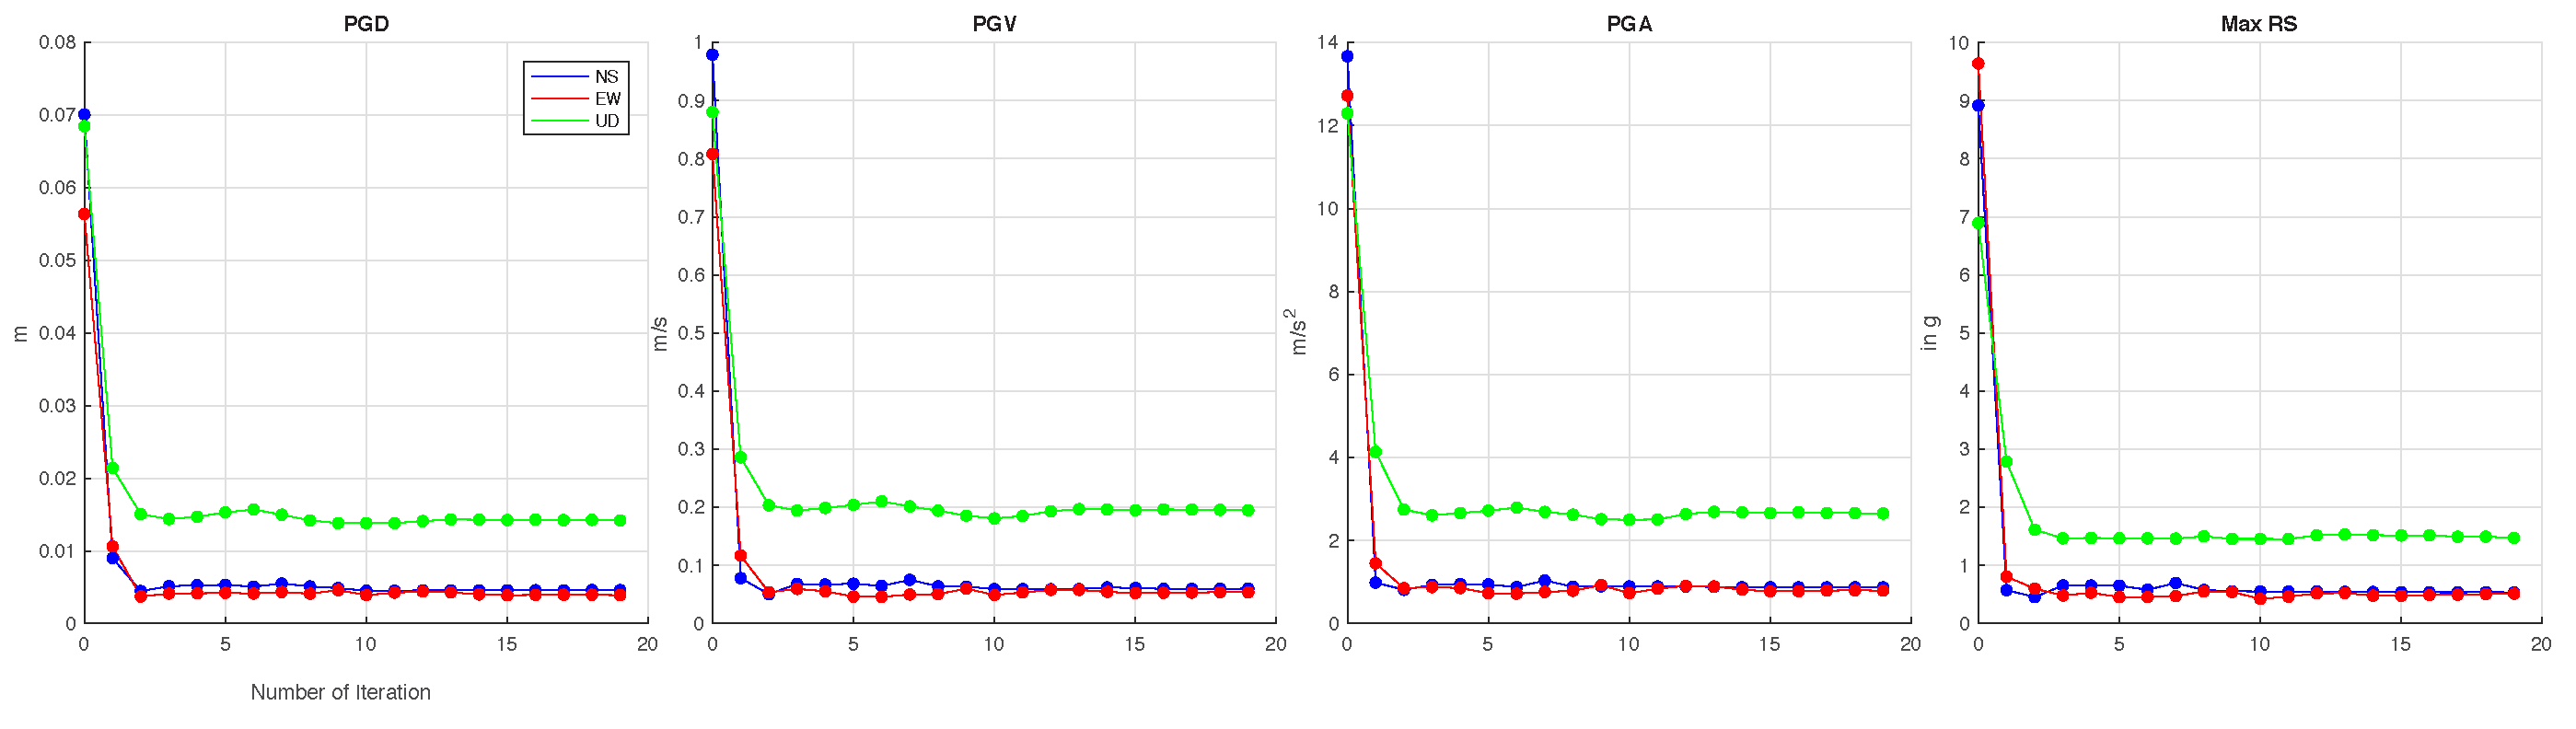
\includegraphics[width=\textwidth]{figures/pdf/iteration_surface.pdf}
    \caption{Analysis of stability of results in different iteration. Stations at the surface of the basin.}
    \label{fig:iteration_surface}
\end{figure}


\begin{figure}
    \centering
    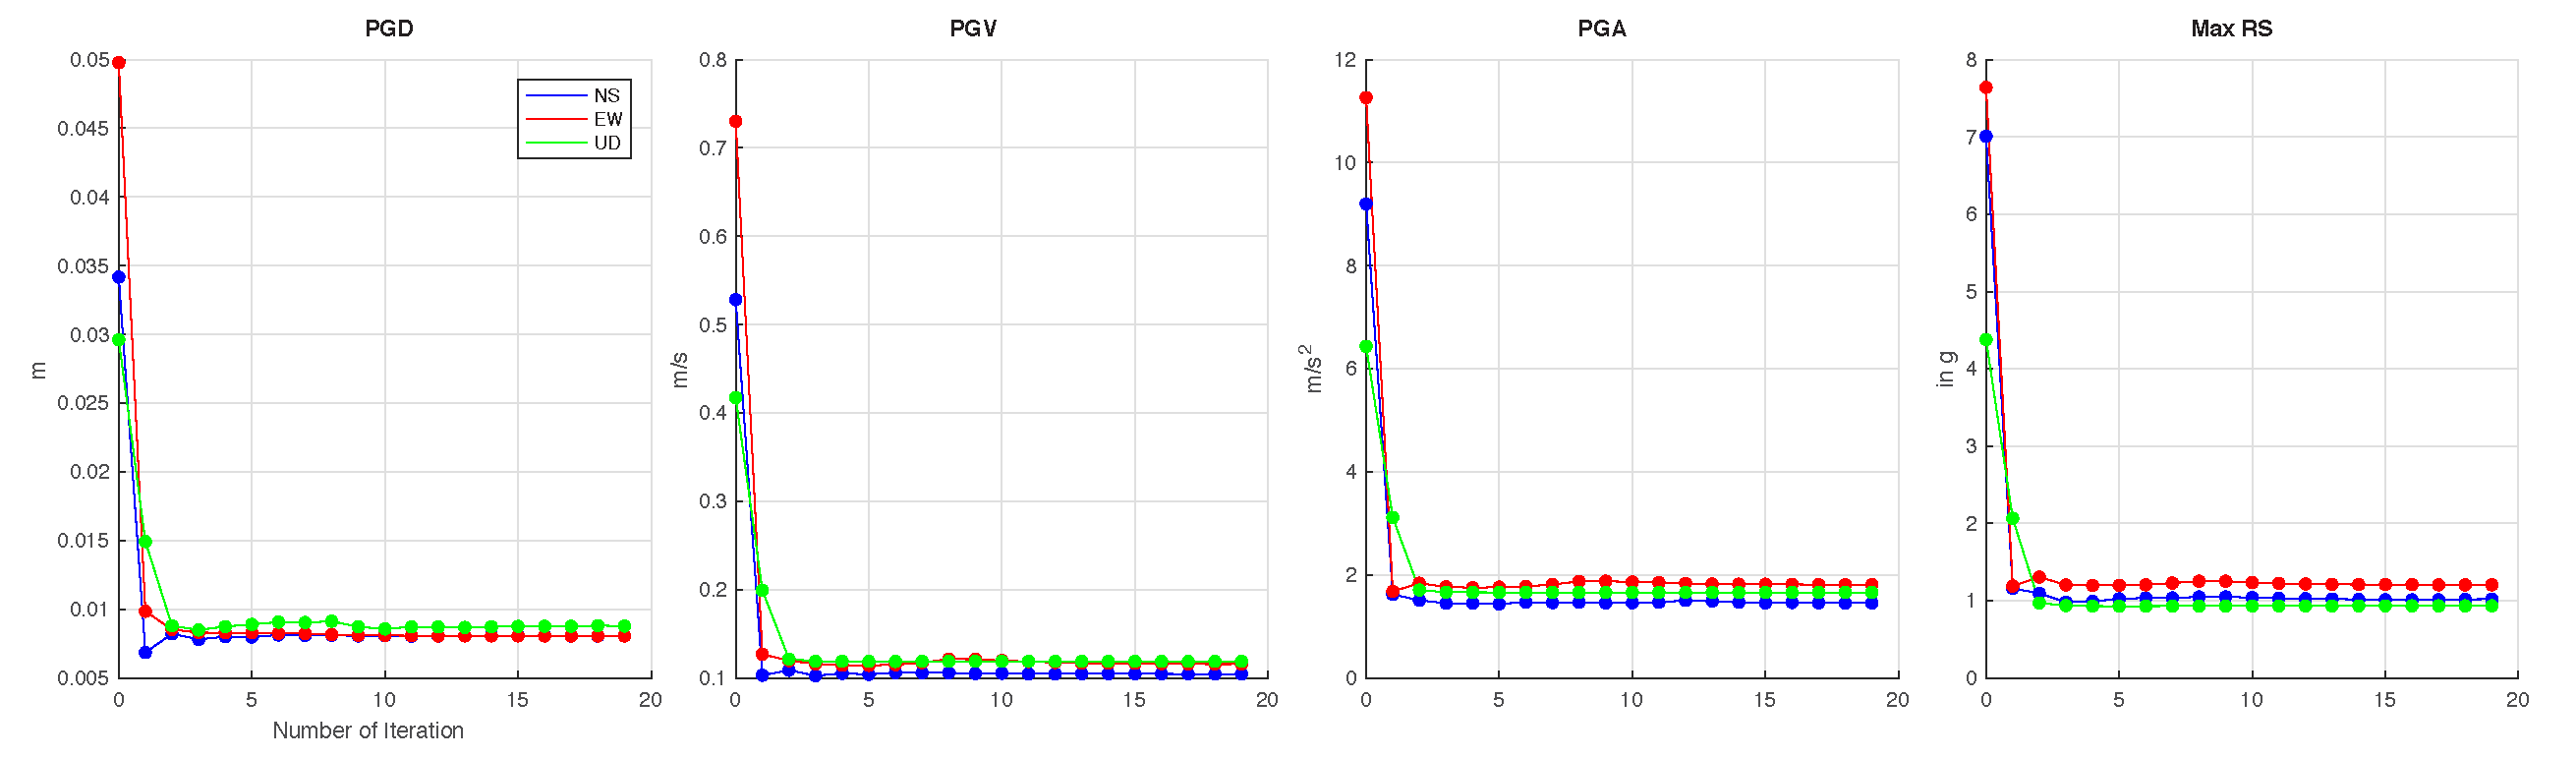
\includegraphics[width=\textwidth]{figures/pdf/iteration_deep_64.pdf}
    \caption{Analysis of stability of results in different iteration. Stations at the depth of 64 m.}
    \label{fig:iteration_deep_64}
\end{figure}




\section{Comparison Metrics}

In this study response spectra is the most important factor to choose the best model. As we discussed the equivalent linear method is a linear process, therefore, the final displacement will not be accurate specially when we have a permanent displacement. Therefore, acceleration and response spectra would be the best options. A simple method to compute the response spectra residuals is subtracting two data and divide them by one of them. 


\begin{equation}
Residual_{Sa} = mean[\frac{Sa_{nonlinear} - Sa_{equivalent linear}}{Sa_{nonlinear}}],
\end{equation}

According to this equation, if nonlinear simulation results is much higher than equivalent linear, then the residual will be close to one, however, if it is much lower, the residual will be a negative number. The problem with this method is its weakness in representing higher residuals in more than 1 for the positive residuals.  Other approaches are mentioned in the literature to compare the response spectra of two waveform. \citet{Anderson_2004_Proc} uses,

\begin{equation}
S_{sa} = mean[S(SA_1(f_j),SA_2(fj))],
\end{equation}

where the average is over all frequencies at which SA is computed in the frequency band being considered. And $S $ defined as,

\begin{equation}
	S( p_1, p_2) = 10 exp \{ - [ \frac{(p_1 - p_2)}{ \min( p_1, p_2 ) }]^2 \},
\end{equation}

The equation, which is used for GOF score, put the scores from comfortable range of values (0-10) regarding the poorest fit and excellent fit. This is a very good scale, however, it can not represent which simulation had a higher values. Because the results are always positive.  \citet{Assimaki2008quantifying} used cumulative normalized error between observation and prediction:

\begin{equation}
e_{SA}=\frac{1}{n}\sqrt{\sum_{i=1}^{n}[\frac{SA_o(T_i)-SA_p(T_i)}{SA_o(T_i)}]^2}
\end{equation}

This metric also represents positive residual values. 

\citet{Assimaki2012} and \citet{Carlton2016comparison} used the following equation to measure of misfit between two $SA$s:

\begin{equation}
e_{SA}^{non}=\mu(e_{SAi})=\mu(log(\frac{SA_{i}^{non}}{SA_{i}^{eq}}))
\end{equation}

This metric can represent a good variation of residuals and does not saturate. Also positive residuals represent higher values for nonlinear and negative values represent higher values for equivalent linear. Fig.~\ref{fig:response_spectra_sensitivity} shows the relationship between these metrics. In this study we use logarithmic residuals. 


\begin{figure}[H]
    \centering
    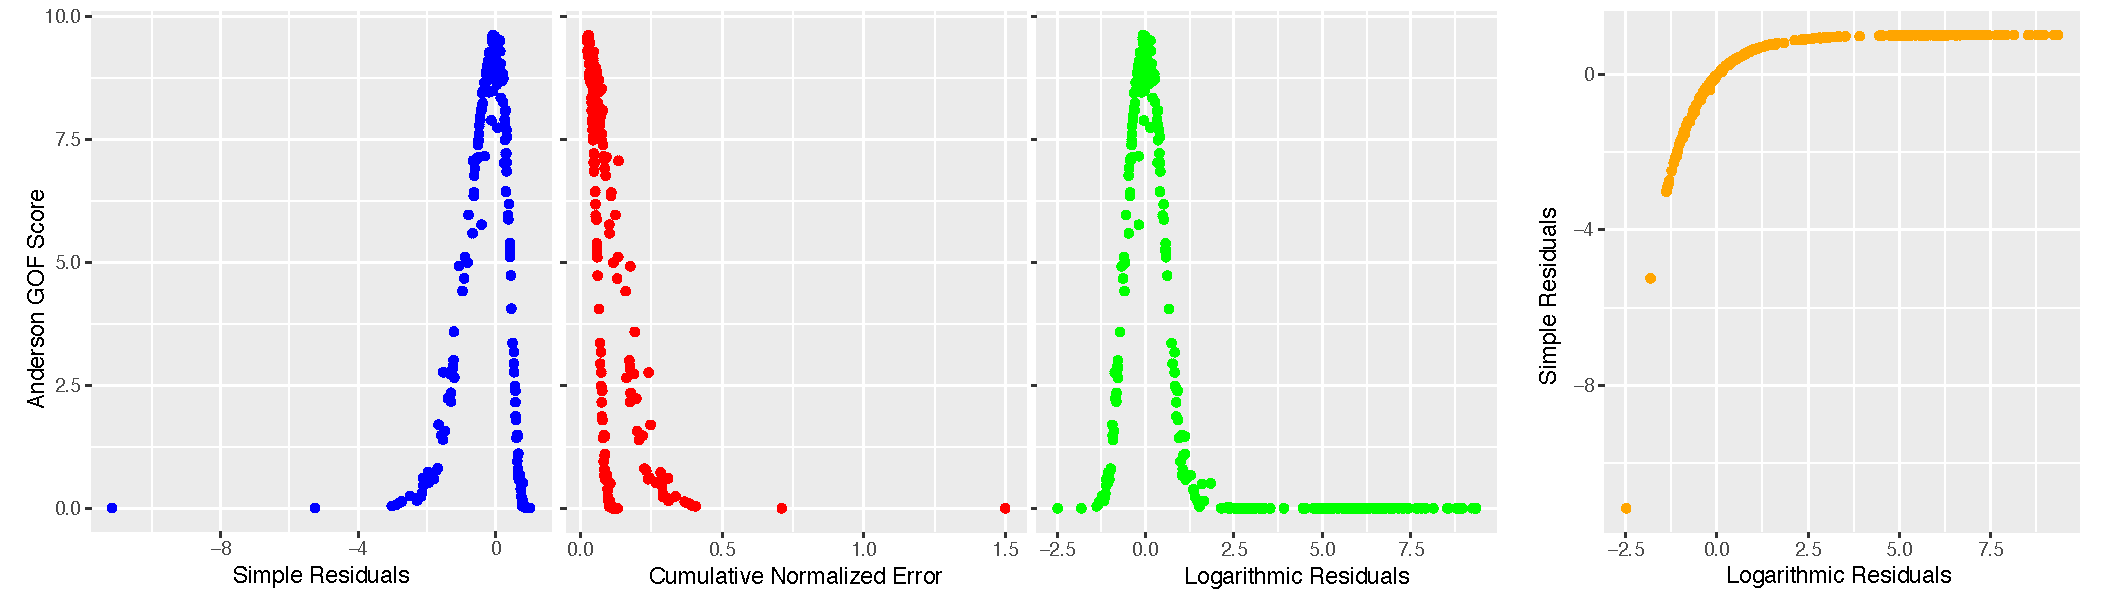
\includegraphics[width=\textwidth]{figures/pdf/response_spectra_sensitivity.pdf}
    \caption{}
    \label{fig:response_spectra_sensitivity}
\end{figure}





\bibliographystyle{spbasic}
\bibliography{references}

% \section{Introduction}
% \label{sec:introduction}
% Your text comes here. Separate text sections with
% \section{Section title}
% \label{sec:1}
% Text with citations \cite{RefB} and \cite{RefJ}.
% \subsection{Subsection title}
% \label{sec:2}
% as required. Don't forget to give each section
% and subsection a unique label (see Sect.~\ref{sec:1}).
% \paragraph{Paragraph headings} Use paragraph headings as needed.
% \begin{equation}
% a^2+b^2=c^2
% \end{equation}

% % For one-column wide figures use
% \begin{figure}
% % Use the relevant command to insert your figure file.
% % For example, with the graphicx package use
%   \includegraphics{example.eps}
% % figure caption is below the figure
% \caption{Please write your figure caption here}
% \label{fig:1}       % Give a unique label
% \end{figure}
% %
% % For two-column wide figures use
% \begin{figure*}
% % Use the relevant command to insert your figure file.
% % For example, with the graphicx package use
%   \includegraphics[width=0.75\textwidth]{example.eps}
% % figure caption is below the figure
% \caption{Please write your figure caption here}
% \label{fig:2}       % Give a unique label
% \end{figure*}
% %
% % For tables use
% \begin{table}
% % table caption is above the table
% \caption{Please write your table caption here}
% \label{tab:1}       % Give a unique label
% % For LaTeX tables use
% \begin{tabular}{lll}
% \hline\noalign{\smallskip}
% first & second & third  \\
% \noalign{\smallskip}\hline\noalign{\smallskip}
% number & number & number \\
% number & number & number \\
% \noalign{\smallskip}\hline
% \end{tabular}
% \end{table}


%\begin{acknowledgements}
%If you'd like to thank anyone, place your comments here
%and remove the percent signs.
%\end{acknowledgements}

% BibTeX users please use one of
%\bibliographystyle{spbasic}      % basic style, author-year citations
%\bibliographystyle{spmpsci}      % mathematics and physical sciences
%\bibliographystyle{spphys}       % APS-like style for physics
%\bibliography{references}   % name your BibTeX data base


% Non-BibTeX users please use
% \begin{thebibliography}{}
% %
% % and use \bibitem to create references. Consult the Instructions
% % for authors for reference list style.
% %
% \bibitem{RefJ}
% % Format for Journal Reference
% Author, Article title, Journal, Volume, page numbers (year)
% % Format for books
% \bibitem{RefB}
% Author, Book title, page numbers. Publisher, place (year)
% % etc
% \end{thebibliography}

\end{document}

